\chapter{Dataset overview}
\section{Introduction}
The dataset used for this project is the \textbf{Kepler Object of Interest (KOI)} dataset, which is a collection of observations of exoplanets provided by \href{https://exoplanetarchive.ipac.caltech.edu/index.html}{NASA's Exoplanet Archive}. In particular, the dataset selected for this statistical analysis aimed at predicting exoplanet status is the Q1-Q17 Data Release 25 (DR 25) Kepler Objects of Interest (KOI) table. This specific table was chosen due to several key characteristics that make it particularly well-suited for developing robust statistical models:

\begin{enumerate}
    \item \textbf{Uniform Data Processing}: The table is derived from Data Release 25, which represents the final, uniform processing of the entire primary Kepler mission dataset (Quarters 1 through 17). This ensures consistency in the underlying light curve data used for analysis.
    \item \textbf{Automated and Uniform Vetting}: A critical feature of the DR 25 KOI table is its use of a fully automated dispositioning process, known as the Kepler Robovetter. This algorithm applies a consistent set of rules and metrics to uniformly classify each Threshold Crossing Event (TCE) as either a Planetary Candidate (PC) or a False Positive (FP).
    \item \textbf{Designed for Statistical Analysis}: As explicitly stated in its documentation, this catalog was generated with the primary goal of enabling statistical analyses, such as the calculation of exoplanetary occurrence rates. The emphasis was placed on uniformity and automated, repeatable classification rather than maximizing the accuracy for every single individual object (which might involve manual intervention or external data, as seen in the DR25 Supplemental table).
    \item \textbf{Homogeneity}: The automated and uniform vetting process yields a homogenous catalog suitable for robust statistical analyses. This internal consistency is crucial for training reliable statistical or machine learning models, as the classification criteria are applied consistently across all entries designated as KOIs within this table.
\end{enumerate}

Therefore, the Q1-Q17 DR 25 KOI table was selected because its **rigorous, automated, and uniform classification methodology provides the most suitable foundation for building a statistical model** intended to predict whether an object is likely an exoplanet based on the parameters derived consistently from the Kepler pipeline and vetting process. This minimizes biases that could arise from aggregating data processed or vetted using different methods over time, as found in the Cumulative table, or from incorporating non-uniform manual assessments, as in the Supplemental table.

\section{An overview of the dataset}
Let's start by understanding what the dataset contains, in particular, what are KOI and the details of each column used in the analysis.

\subsection{Kepler Object of Interest (KOI)}
A \textbf{Kepler Object of Interest (KOI)} is a target star observed by NASA's Kepler space telescope that exhibits transit-like signals in its photometric light curve data. These signals meet specific criteria suggesting they might be caused by an object passing in front of (transiting) the star, with characteristics initially consistent with those of an exoplanet.

Specifically, a target star receives a KOI designation when:
\begin{itemize}
    \item Its Kepler light curve shows at least one sequence of periodic, transit-like dips in brightness.
    \item The detected signal appears to be of astrophysical origin, rather than being caused by instrumental effects or stellar variability that only mimics a transit.
    \item The signal's properties (like shape, duration, and depth) are initially consistent with the hypothesis of a planet passing in front of its host star.
\end{itemize}

Each potential transiting object identified is assigned a unique KOI name, typically in the format KIC\_Number.XX or KOI-Number.XX (e.g., K00752.01 or KOI-752.01). The integer part refers to the target star (often linked to its Kepler Input Catalog or KIC number), and the two-digit decimal part identifies a specific transit signature associated with that star (allowing for multi-planet systems).

It is crucial to understand that a KOI designation represents a \textit{candidate} detection. It signifies that an interesting signal worthy of further investigation has been found, but it does not guarantee the presence of a planet. Every KOI must undergo a rigorous vetting process, utilizing detailed analysis of the Kepler pixel data, light curves, and often supplementary follow-up observations from other telescopes. This vetting aims to classify each KOI into more definitive categories:

\begin{itemize}
    \item \textbf{Planetary Candidate (PC):} A KOI that successfully passes all vetting tests designed to rule out common false positive scenarios. It remains consistent with being a genuine planet, pending further confirmation.
    \item \textbf{False Positive (FP):} A KOI whose signal is ultimately determined to be caused by something other than a transiting planet. Common sources of false positives include eclipsing binary star systems (within the target aperture or in the background), stellar variability (like starspots), or instrumental artifacts.
    \item \textbf{Confirmed Planet:} A Planetary Candidate that has been statistically validated or independently confirmed as a planet through methods such as measuring its mass (via radial velocity or transit timing variations) or achieving extremely high confidence through statistical analysis. Confirmed planets typically receive official names (e.g., Kepler-186f).
\end{itemize}

The various KOI catalogs released by the Kepler mission team are foundational datasets for the exoplanet community. They provide lists of targets for detailed follow-up observations and serve as the basis for statistical studies aimed at understanding the prevalence and characteristics of planets beyond our solar system (planet occurrence rates).

\subsection{Feature Description}
The dataset contains 8054 rows and 142 columns, each row representing a different object and each column representing a different parameter. The following is a list of the most important columns and their description:
\begin{itemize}
    \item \texttt{koi\_period} - \textbf{Orbital Period (days):} Time interval between consecutive transits.
    \item \texttt{koi\_duration} - \textbf{Transit Duration (hours):} Duration of the transit event from first to last contact.
    \item \texttt{koi\_depth} - \textbf{Transit Depth (ppm):} Maximum fractional decrease in stellar flux during transit (parts per million).
    \item \texttt{koi\_prad} - \textbf{Planetary Radius (Earth radii):} Estimated radius of the KOI (R$_{\oplus}$).
    \item \texttt{koi\_teq} - \textbf{Equilibrium Temperature (Kelvin):} Estimated temperature assuming typical albedo and heat redistribution (K).
    \item \texttt{koi\_insol} - \textbf{Insolation Flux (Earth flux):} Incident stellar flux relative to Earth.
    \item \texttt{koi\_model\_snr} - \textbf{Transit Signal-to-Noise Ratio:} SNR of the transit detection from model fit.
    \item \texttt{koi\_steff} - \textbf{Stellar Effective Temperature (Kelvin):} Host star's photospheric temperature (K).
    \item \texttt{koi\_slogg} - \textbf{Stellar Surface Gravity (log10(cm s$^{-2}$)):} Log base-10 of the star's surface gravity.
    \item \texttt{koi\_srad} - \textbf{Stellar Radius (solar radii):} Host star's estimated photospheric radius (R$_{\odot}$).
    \item \texttt{koi\_smass} - \textbf{Stellar Mass (solar mass):} Host star's estimated mass (M$_{\odot}$).
    \item \texttt{koi\_impact} - \textbf{Impact Parameter:} Normalized projected distance between star and KOI centers at mid-transit (Dimensionless).
    \item \texttt{koi\_ror} - \textbf{Planet-Star Radius Ratio:} Ratio of KOI radius to stellar radius (Dimensionless).
    \item \texttt{koi\_srho} - \textbf{Fitted Stellar Density (g cm$^{-3}$):} Mean stellar density inferred from transit shape (g cm$^{-3}$).
    \item \texttt{koi\_sma} - \textbf{Orbit Semi-Major Axis (AU):} Half the longest diameter of the orbit (AU).
    \item \texttt{koi\_incl} - \textbf{Inclination (degrees):} Angle between the orbital plane and the plane of the sky.
    \item \texttt{koi\_dor} - \textbf{Planet-Star Distance over Star Radius:} Distance at mid-transit normalized by stellar radius (Dimensionless).
    \item \texttt{koi\_ldm\_coeff1} - \textbf{Limb Darkening Coefficient 1:} First coefficient for the limb darkening model used in the fit.
    \item \texttt{koi\_ldm\_coeff2} - \textbf{Limb Darkening Coefficient 2:} Second coefficient for the limb darkening model used in the fit.
    \item \texttt{koi\_smet} - \textbf{Stellar Metallicity ([Fe/H]):} Log base-10 of the Fe/H ratio relative to solar (dex).
\end{itemize}

\subsection{Target Variable Description}
\texttt{koi\_pdisposition} (\textbf{Disposition Using Kepler Data (Pipeline Disposition)}) is the target variable used for classification in this analysis. It represents the classification assigned to the Kepler Object of Interest (KOI) by the Kepler data processing pipeline and associated automated vetting procedures (like the Robovetter for DR25). It indicates the pipeline's assessment of the most probable physical nature of the transit-like signal based solely on the analysis of Kepler photometric data. The typical values are:
\begin{itemize}
    \item \textbf{CANDIDATE:} The signal passed the automated vetting tests designed to identify common false positives. It remains consistent with the hypothesis of a transiting planet based on the pipeline's analysis.
    \item \textbf{FALSE POSITIVE:} The signal failed at least one vetting test, suggesting it is likely caused by phenomena other than a transiting planet (e.g., an eclipsing binary star system, instrumental artifact, background contamination).
\end{itemize}
This disposition may differ from the final classification in the Exoplanet Archive (\texttt{koi\_disposition}), which incorporates additional information, including human vetting and follow-up observations. For modeling based purely on pipeline-derived features, \texttt{koi\_pdisposition} is often used as the ground truth label.

\chapter{Analysis}
\section{Data preprocessing}
In the \texttt{data\_preparation.rmd} file, the dataset is cleaned from rows with a high rate of missing values and factor variables are prepared for further analysis. Then in the \texttt{data\_visualization.rmd} file, the dataset is visualized to understand the distribution of the variables and the relationship between them.
\subsection{Correlation matrix}
The following is the correlation matrix of the used columns for the analysis. The correlation matrix shows us that there are some strong relationships between some variables and will help us to understand the dataset better.
\begin{figure}[H]
    \centering
    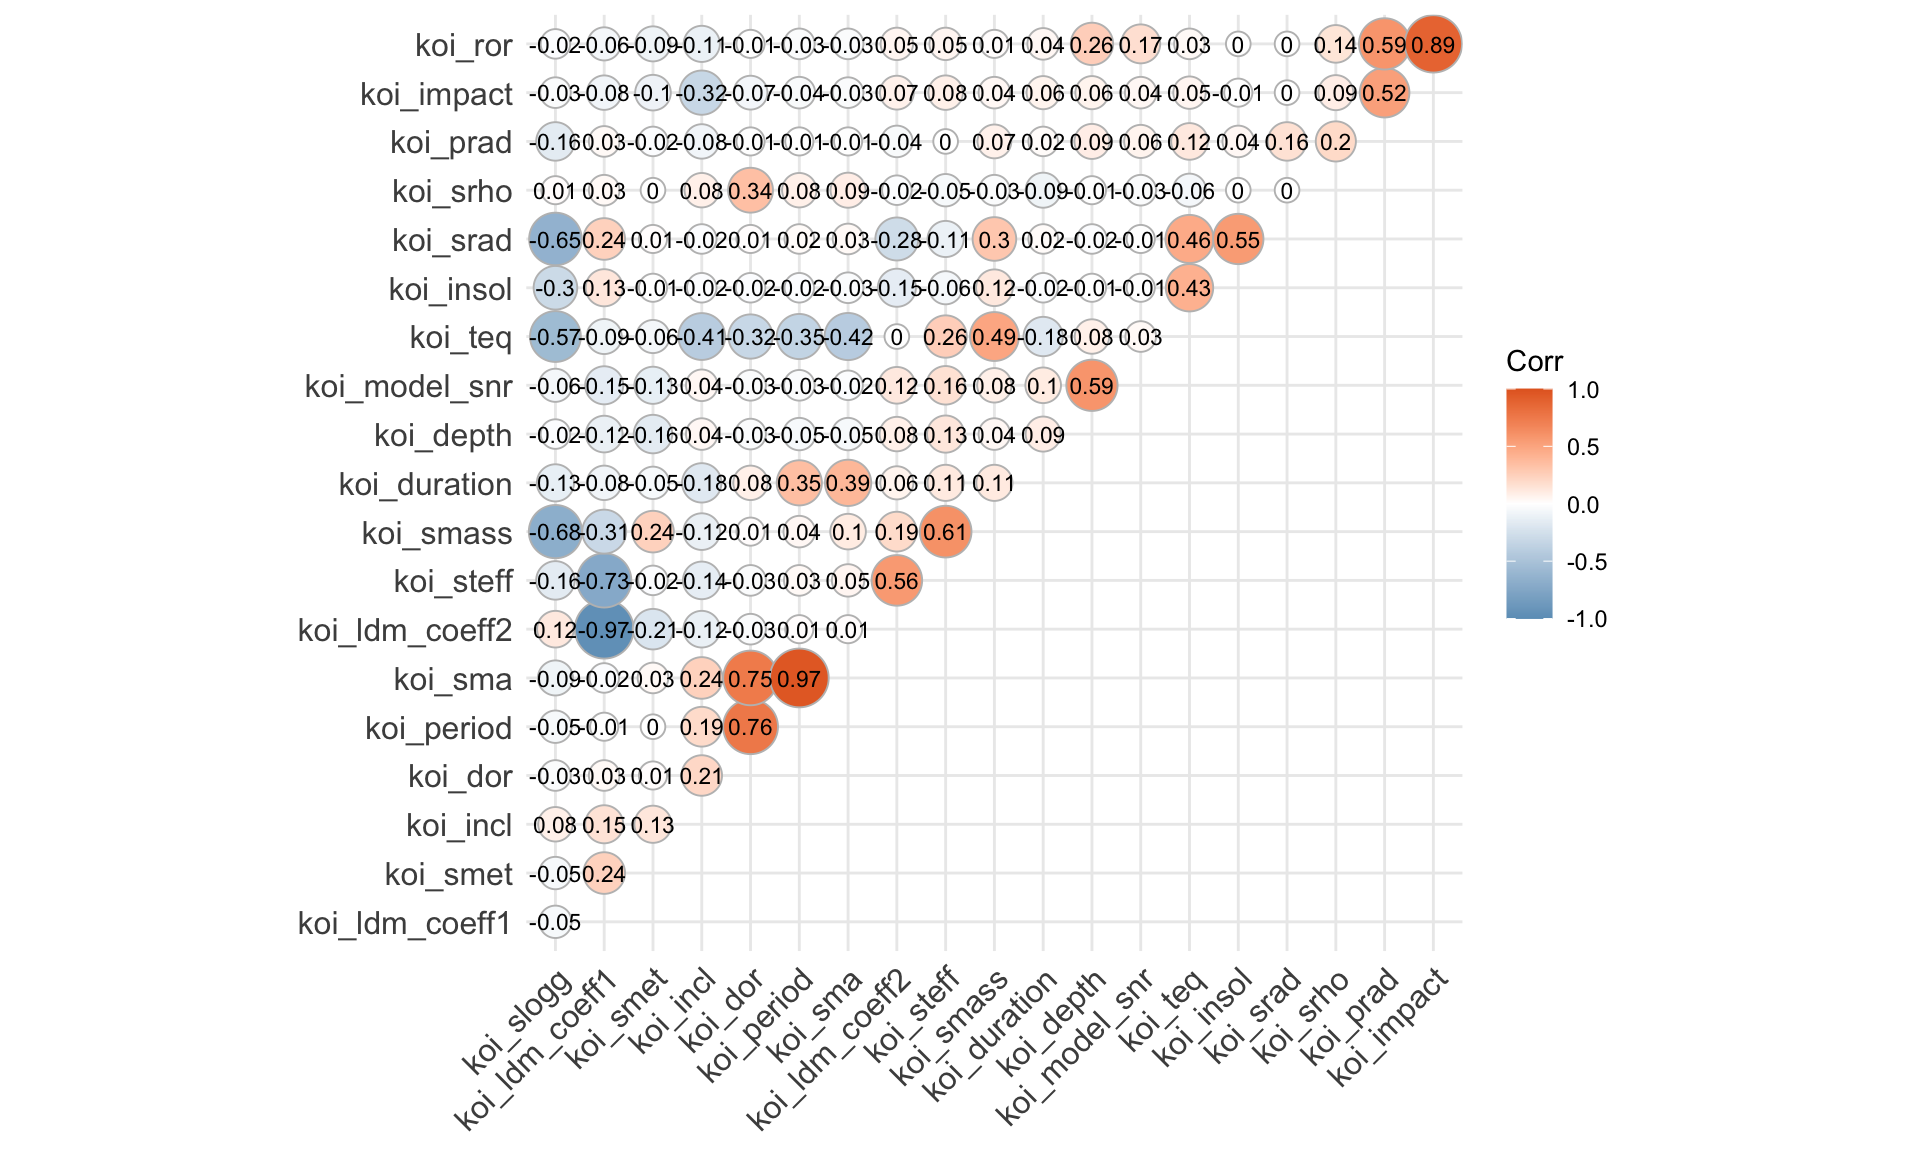
\includegraphics[width=0.9\textwidth]{Immagini/cm.png}
    \caption{Correlation Matrix}
\end{figure}

\section{Visualizations}
The following plots illustrate the distribution of the variables and their relationships based on the used columns for analysis.

\begin{figure}[H]
    \centering
    \begin{subfigure}[b]{0.45\textwidth}
        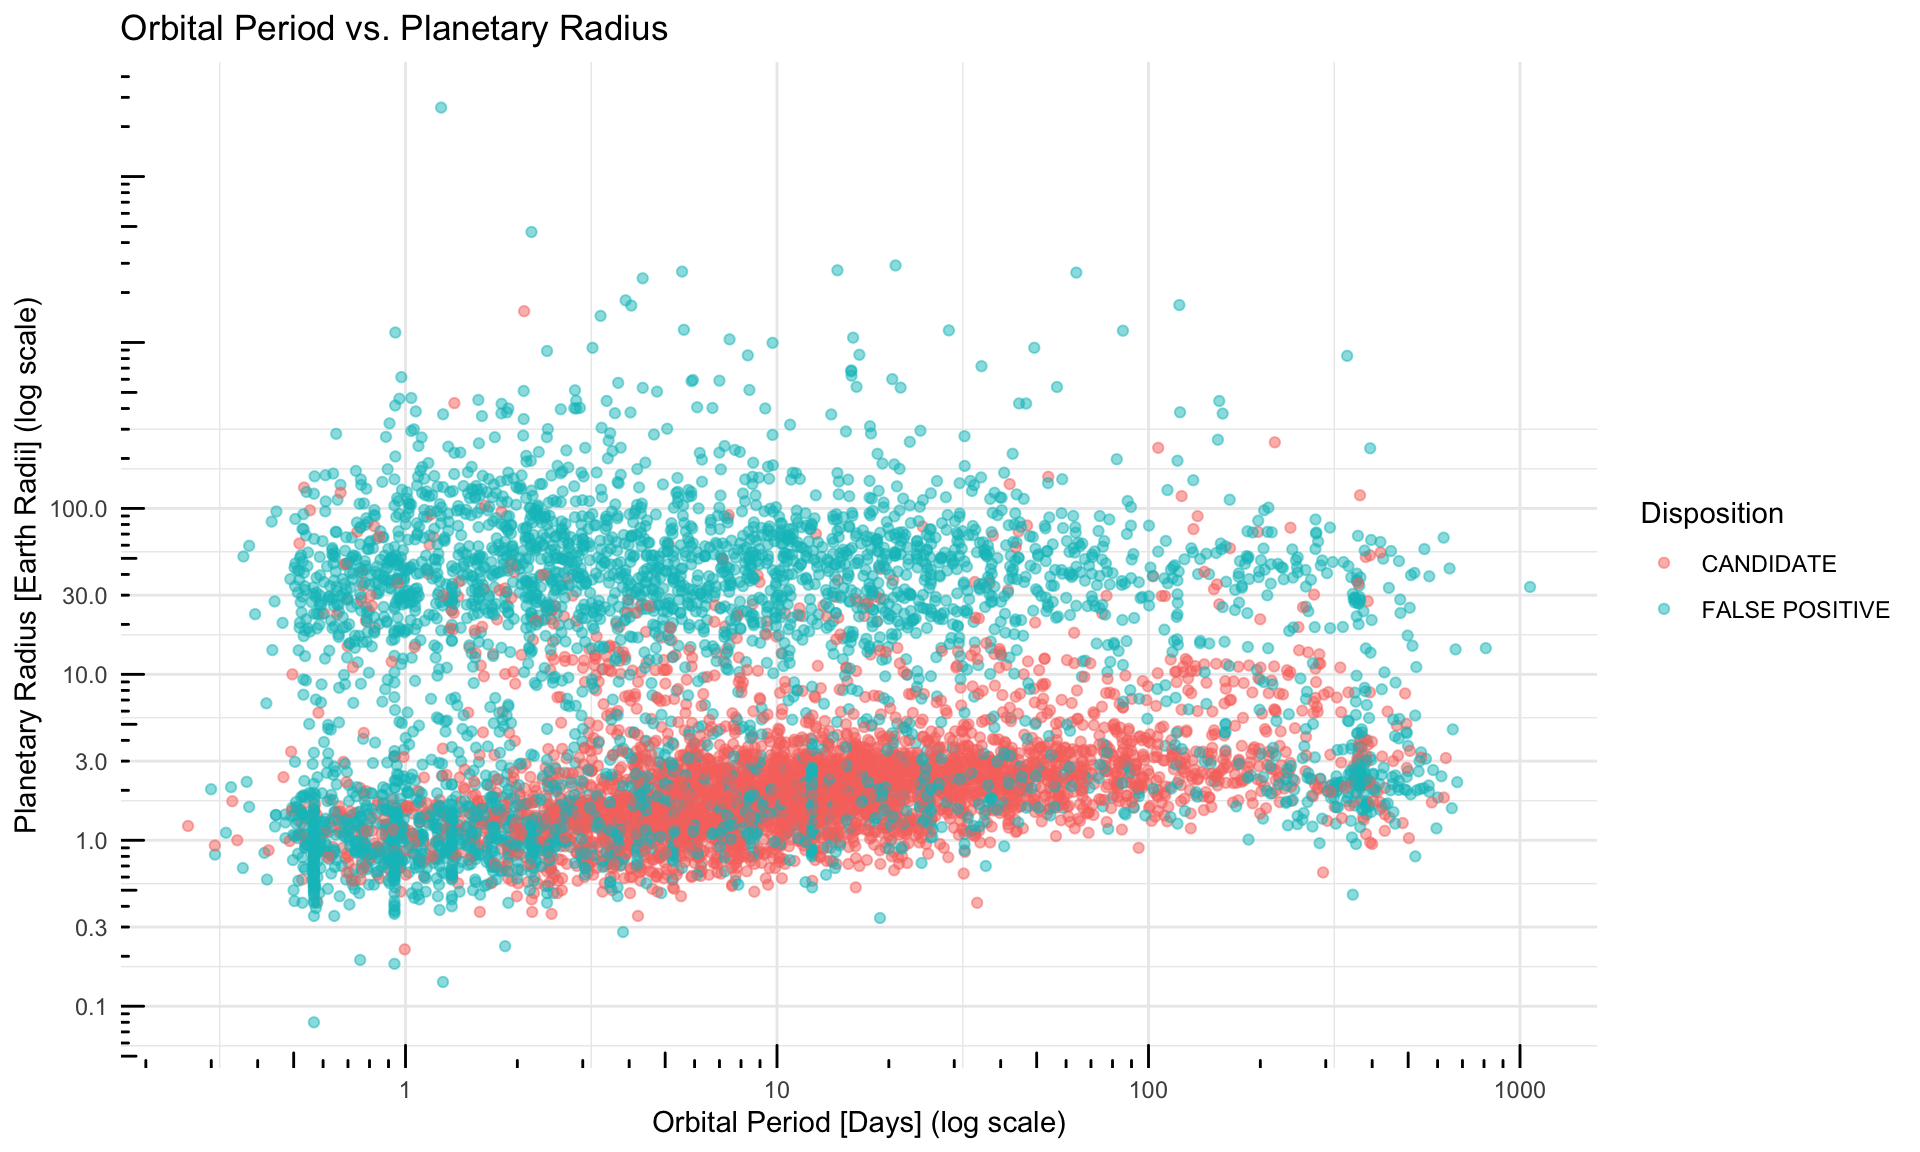
\includegraphics[width=\textwidth]{Immagini/orbital_radius.png}
        \caption{Orbital Period vs. Planetary Radius}
    \end{subfigure}
    \begin{subfigure}[b]{0.45\textwidth}
        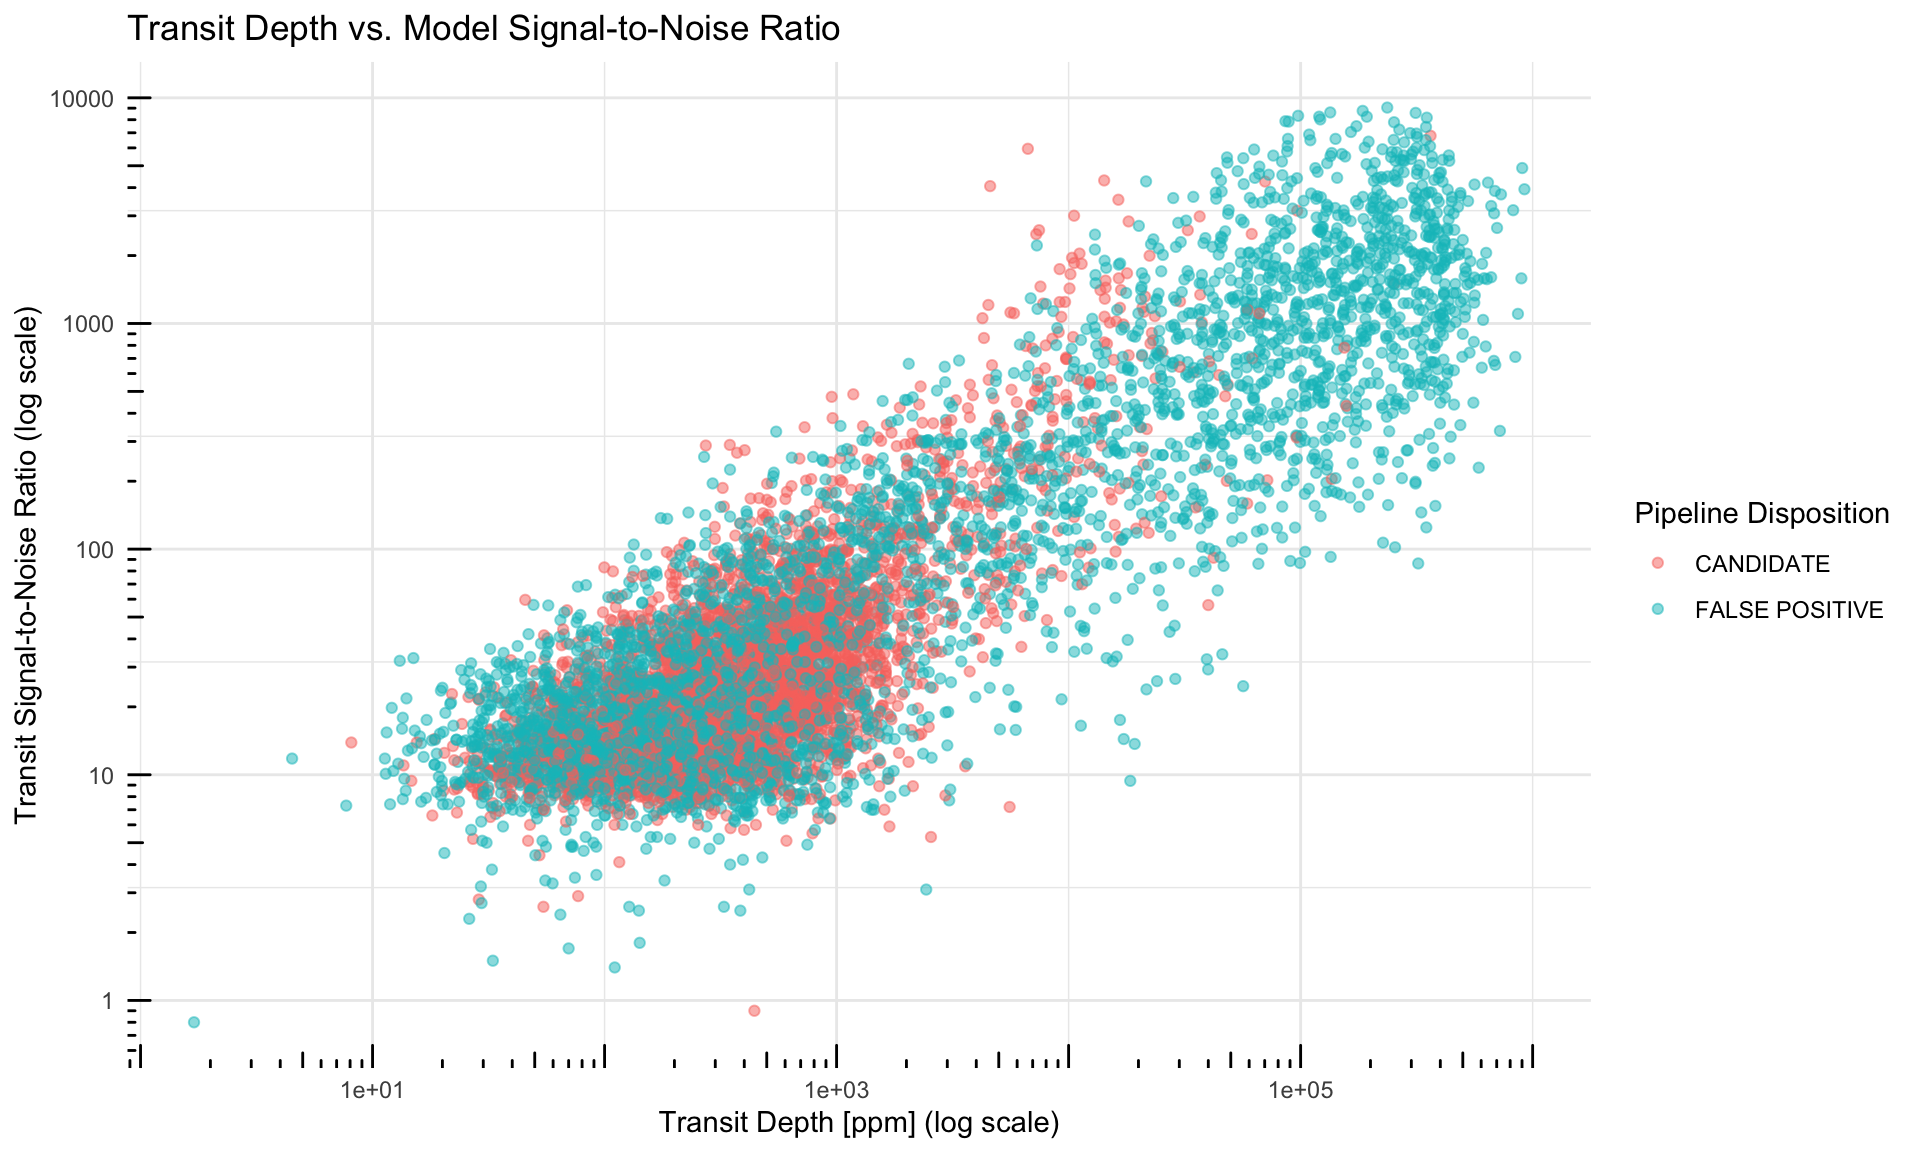
\includegraphics[width=\textwidth]{Immagini/transit_depth.png}
        \caption{Transit Depth vs. Model Signal-to-Noise Ratio}
    \end{subfigure}

    \vspace{0.5cm}
    
    \begin{subfigure}[b]{0.45\textwidth}
        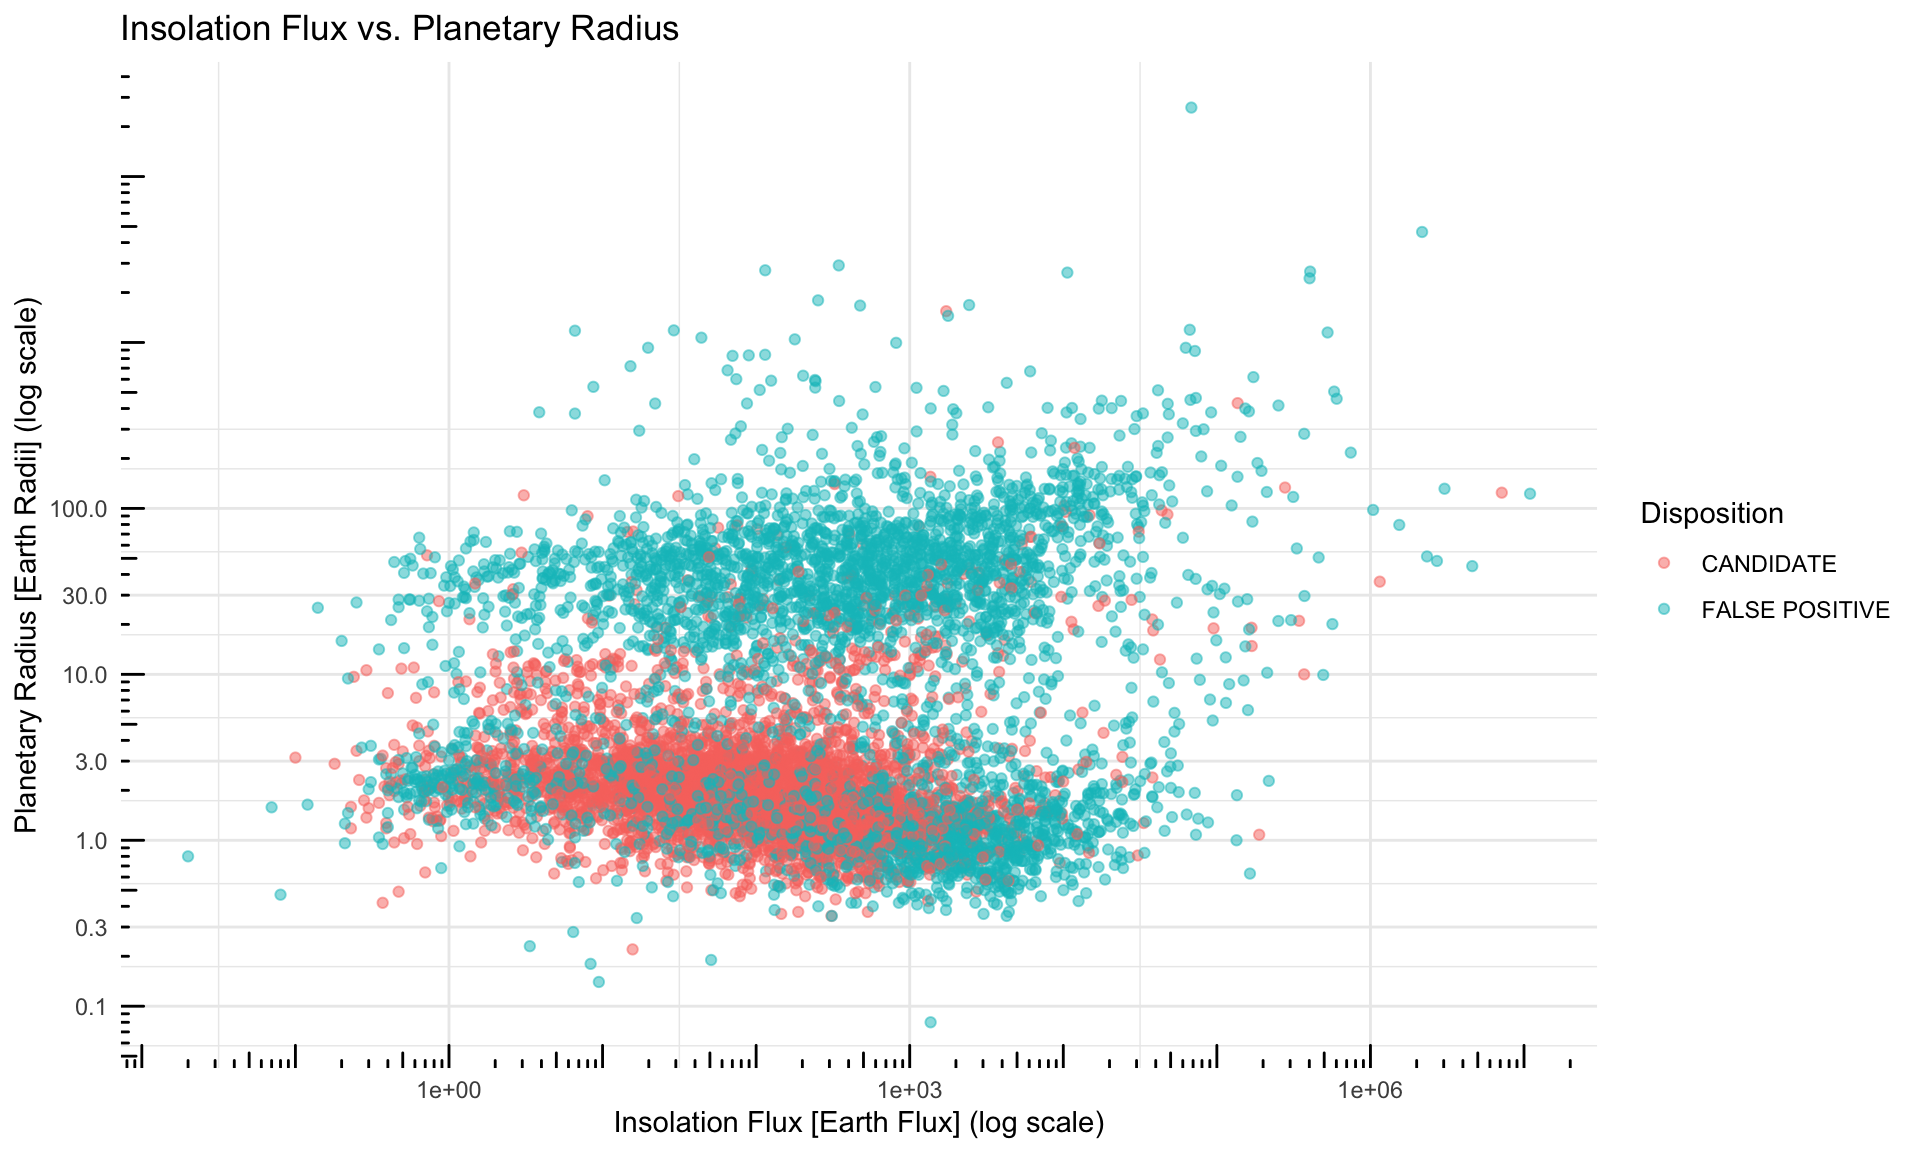
\includegraphics[width=\textwidth]{Immagini/flux_radius.png}
        \caption{Insolation Flux vs. Planetary Radius}
    \end{subfigure}
    \begin{subfigure}[b]{0.45\textwidth}
        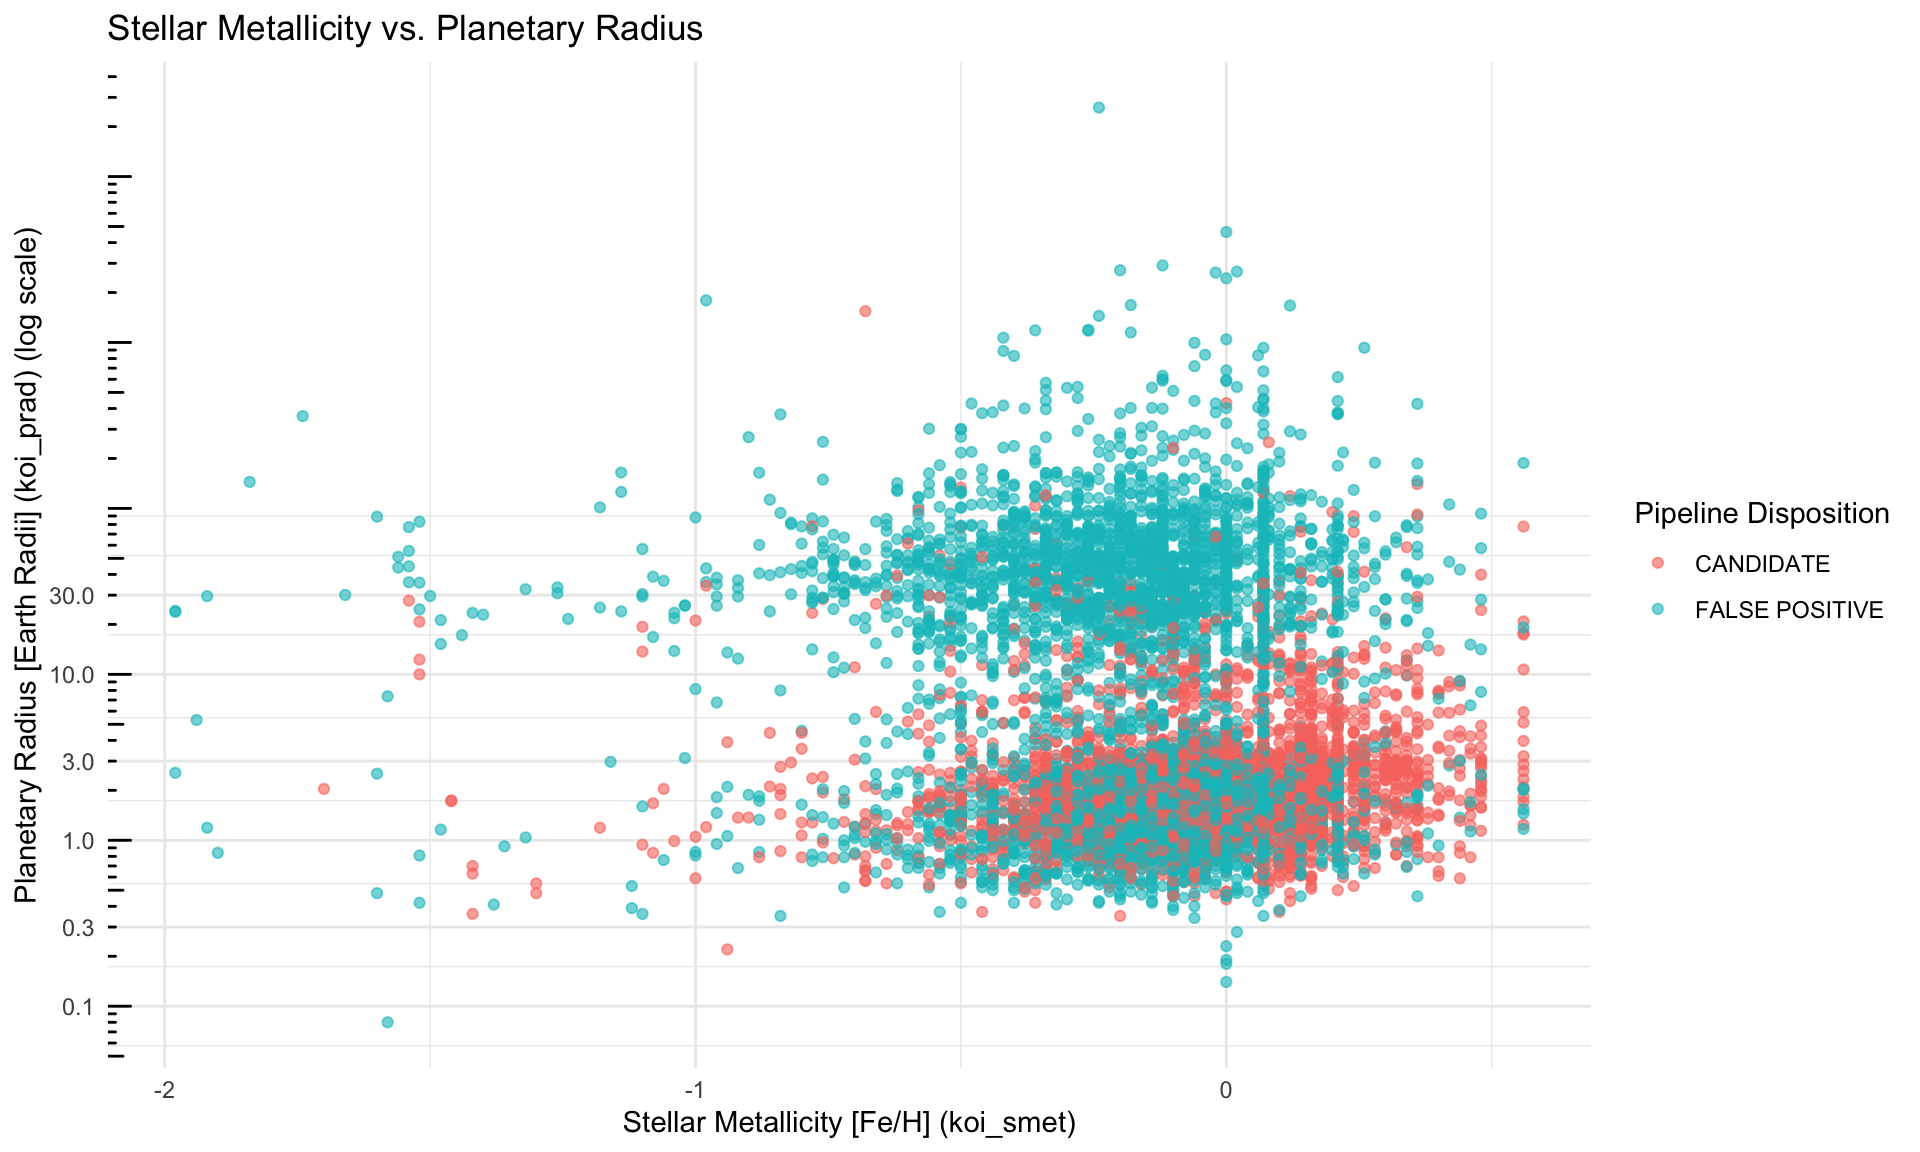
\includegraphics[width=\textwidth]{Immagini/metallicity.png}
        \caption{Stellar Metallicity vs. Planetary Radius}
    \end{subfigure}
    
    \vspace{0.5cm}
    
    \begin{subfigure}[b]{0.3\textwidth}
        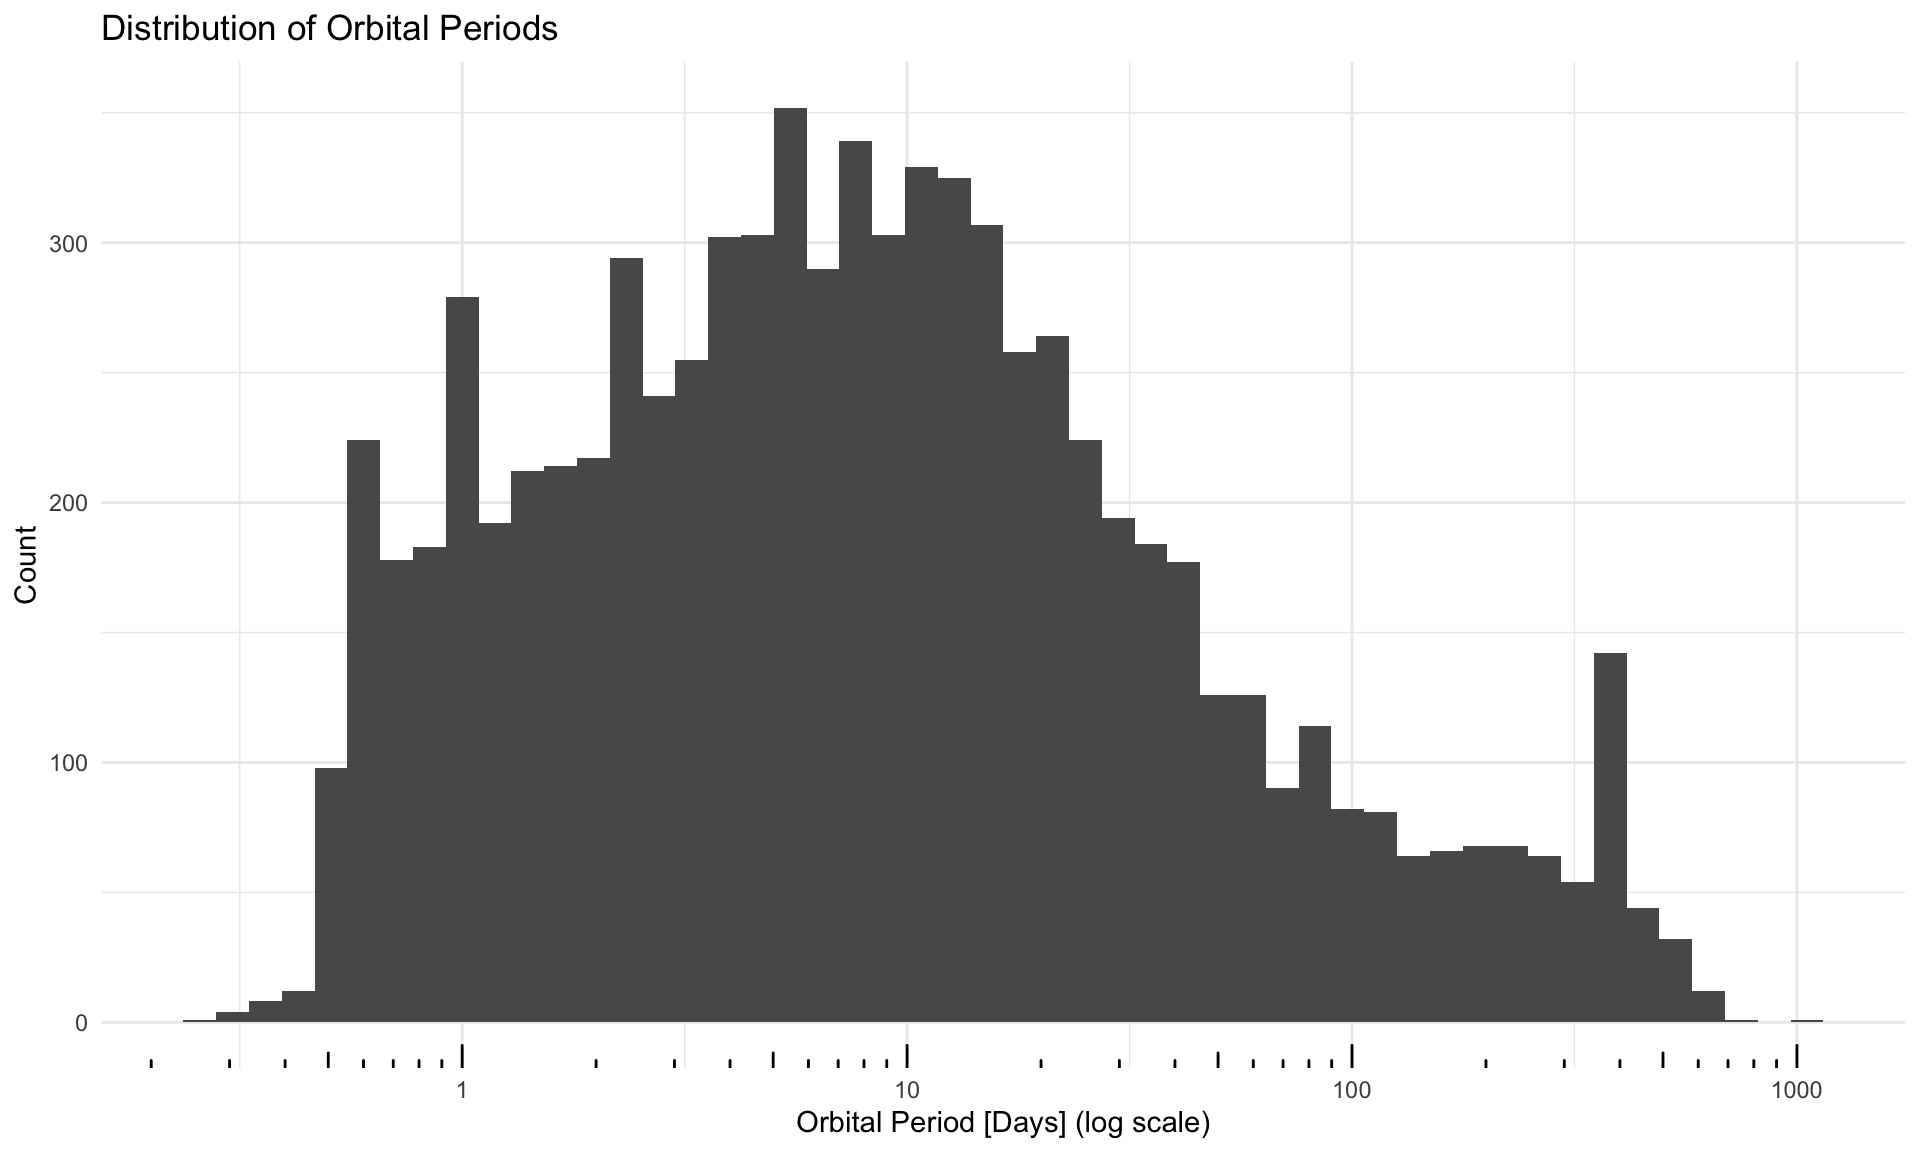
\includegraphics[width=\textwidth]{Immagini/dist_orbital_periods.png}
        \caption{Distribution of Orbital Periods}
    \end{subfigure}
    \begin{subfigure}[b]{0.3\textwidth}
        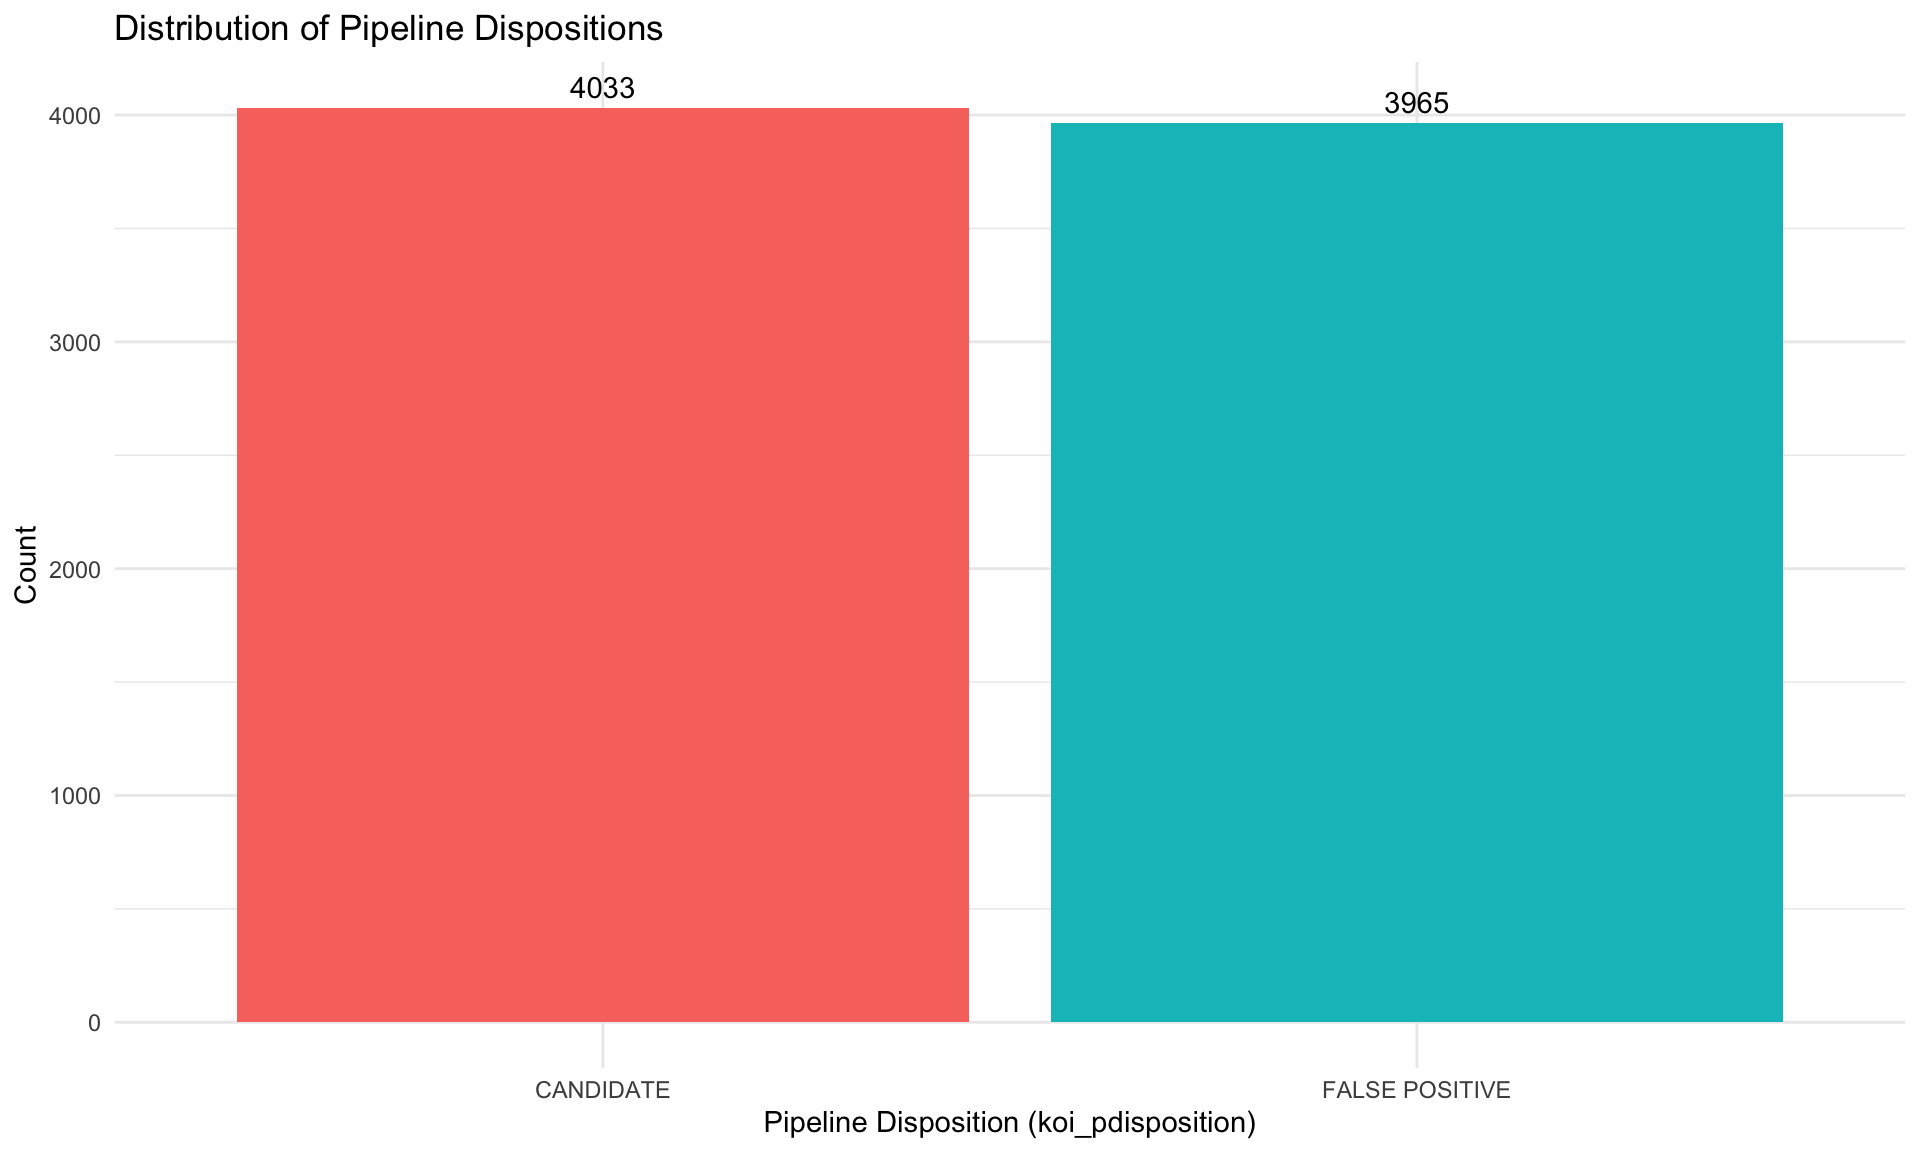
\includegraphics[width=\textwidth]{Immagini/pdisp_dist.png}
        \caption{Distribution of Pipeline Dispositions}
    \end{subfigure}
    \begin{subfigure}[b]{0.3\textwidth}
        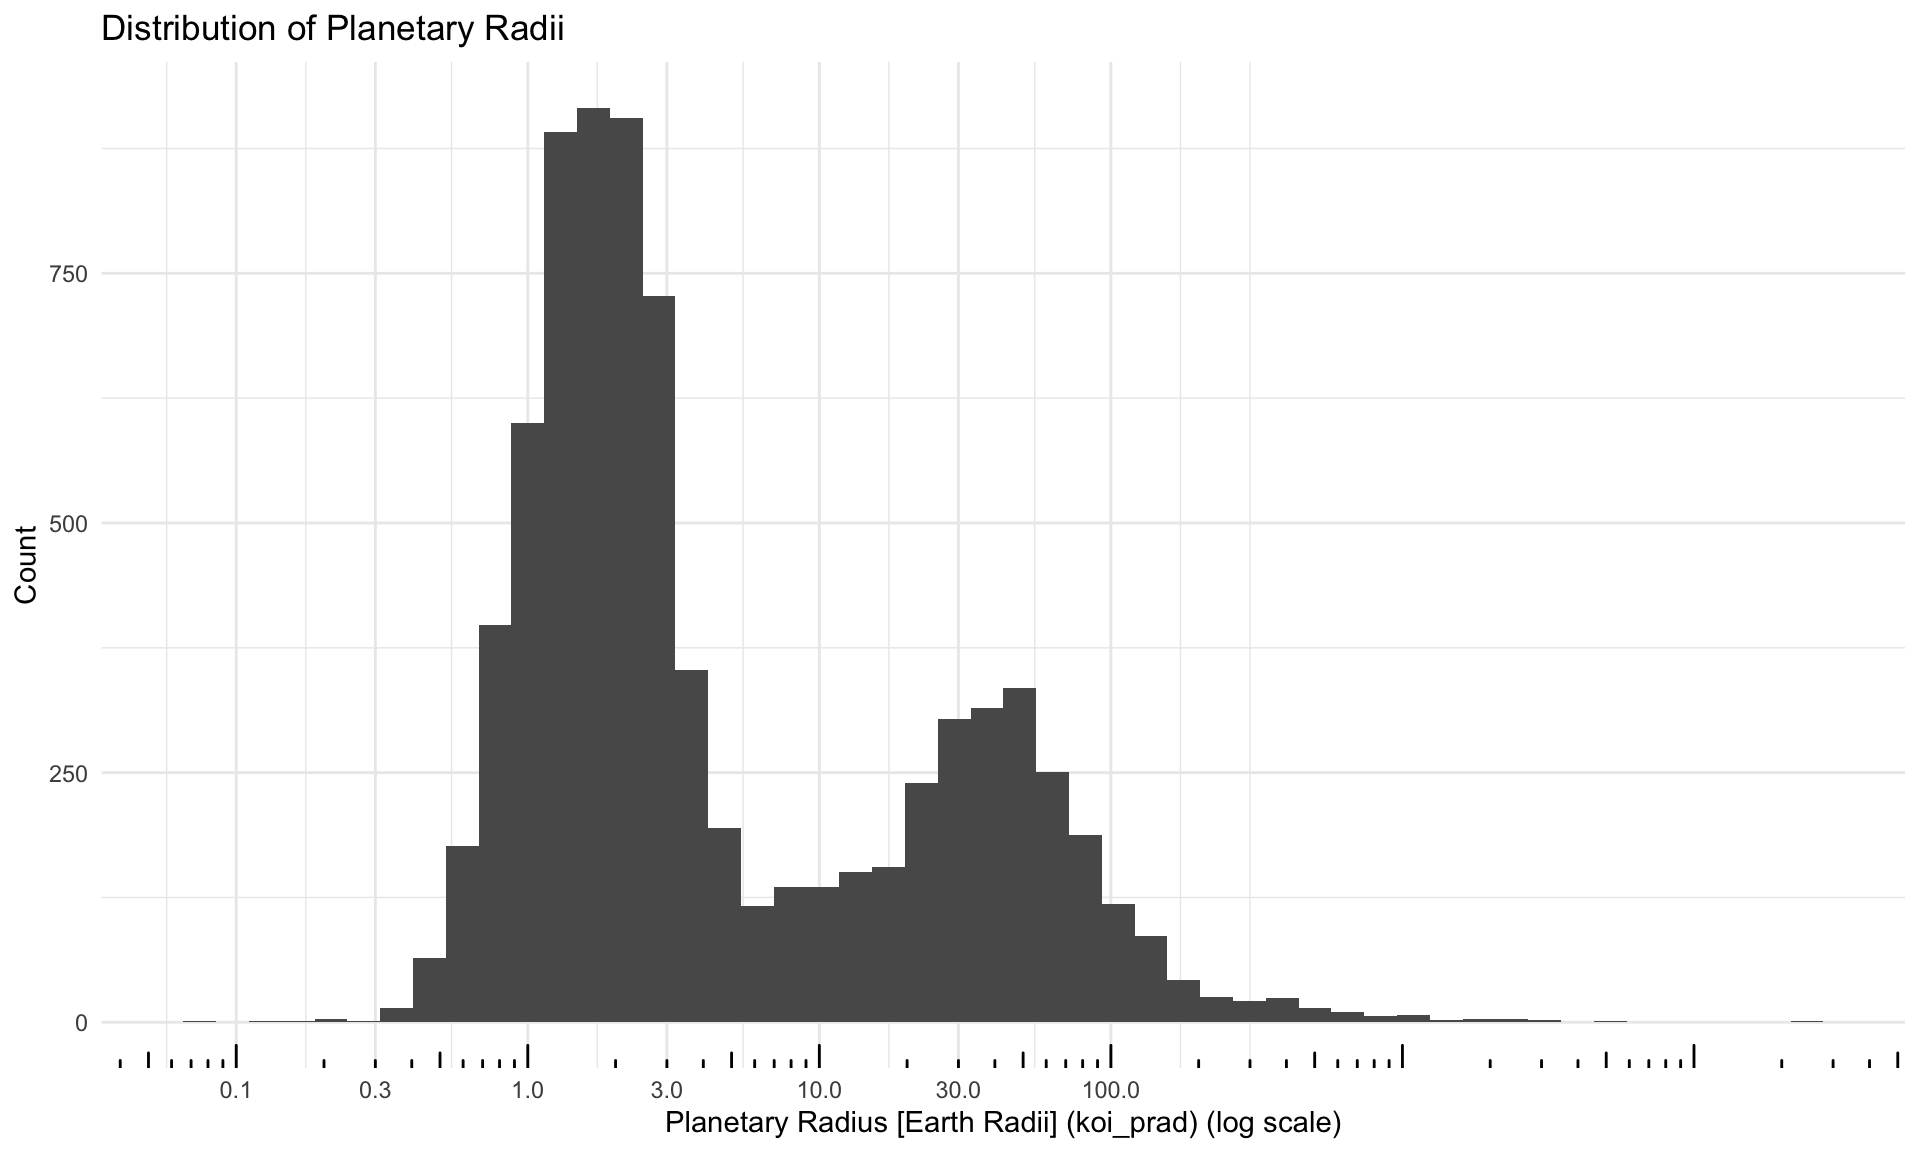
\includegraphics[width=\textwidth]{Immagini/dist_radius.png}
        \caption{Distribution of Planetary Radius}
    \end{subfigure}
    \caption{Distribution of variables and relationships between them.}
    \label{fig:plots_grid}
\end{figure}

\begin{itemize}
    \item \textbf{Orbital Period vs. Planetary Radius:} The plot shows planet radius against orbital period, highlighting known exoplanet populations and false positives.
    \item \textbf{Transit Depth vs. Model Signal-to-Noise Ratio:} Transit depth and SNR are positively correlated, with deeper transits being easier to detect. The plot visualizes false positives and candidates spanning a wide range of depths and SNRs.
    \item \textbf{Insolation Flux vs. Planetary Radius:} The plot examines the relationship between planetary energy receipt, size, and insolation, potentially identifying false positives based on these parameters.
    \item \textbf{Stellar Metallicity vs. Planetary Radius:} The plot investigates the relationship between planet size and star metallicity, examining if CANDIDATEs and FALSE POSITIVEs exhibit distinct trends in this parameter space.
    \item \textbf{Distribution of Orbital Periods:} Most detected KOIs have short orbital periods due to detection bias.
    \item \textbf{Distribution of Pipeline Dispositions:} The plot shows the balance between candidate and false positive KOIs in the Kepler dataset, which is important for model building and evaluation.
    \item \textbf{Distribution of Planetary Radius:} The histogram shows planet candidate sizes, with peaks for common types and a potential dip around 1.5-2 Earth radii. Detection biases influence the distribution.
\end{itemize}

\section{Principal Component Analysis}
Principal Component Analysis (PCA) is a dimensionality reduction technique used to transform a large set of variables into a smaller set of uncorrelated variables called principal components. These principal components are linear combinations of the original variables and capture the maximum amount of variance in the data. PCA is particularly useful when dealing with high-dimensional data, where many variables are correlated. The analysis of the PCA results is performed in the \texttt{data\_visualization.rmd} file and then used to build the models in the \texttt{model\_pca.rmd} file. 

\begin{figure}[H]
    \centering
    \begin{subfigure}[b]{0.49\textwidth}
        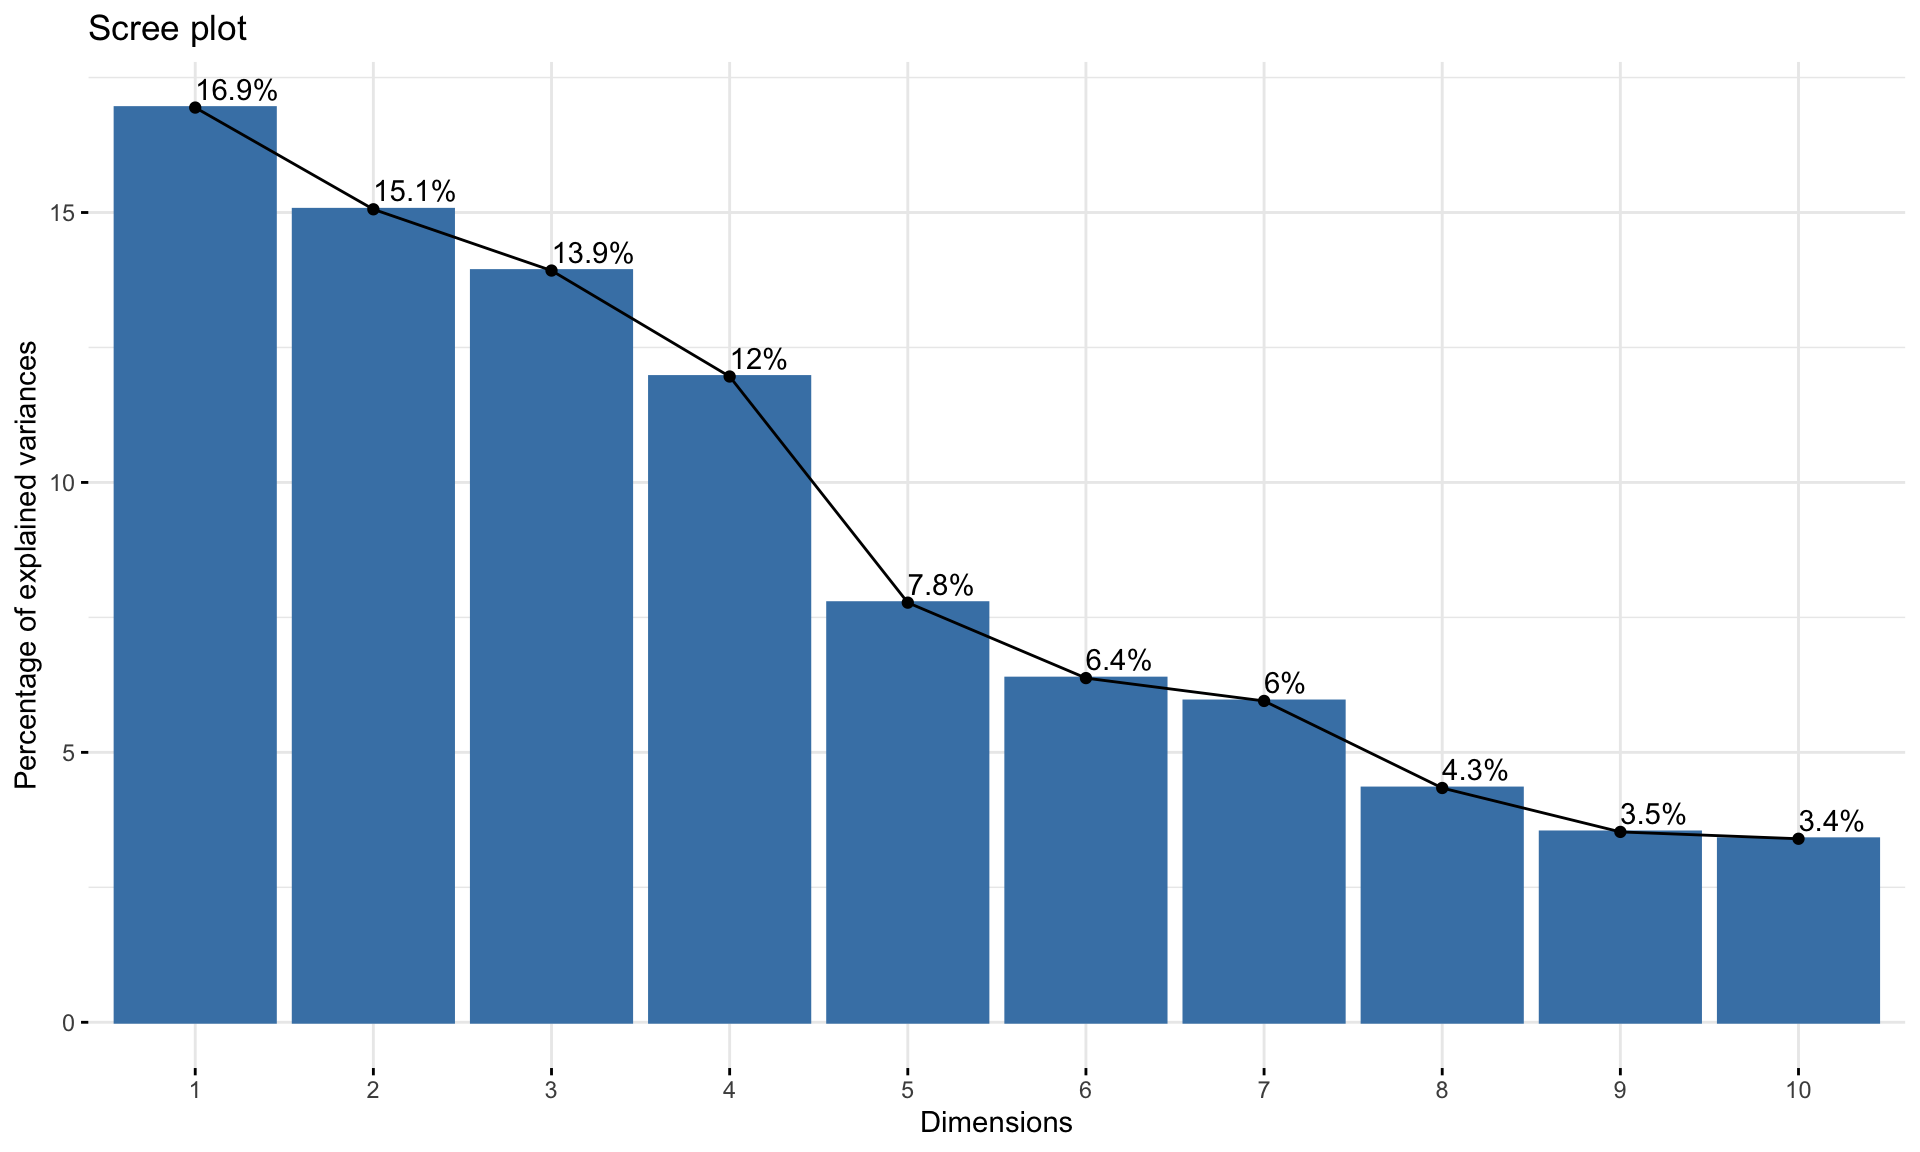
\includegraphics[width=\textwidth]{Immagini/PCA_res.png}
        \caption{PCA eigenvalues}
    \end{subfigure}
    \begin{subfigure}[b]{0.49\textwidth}
        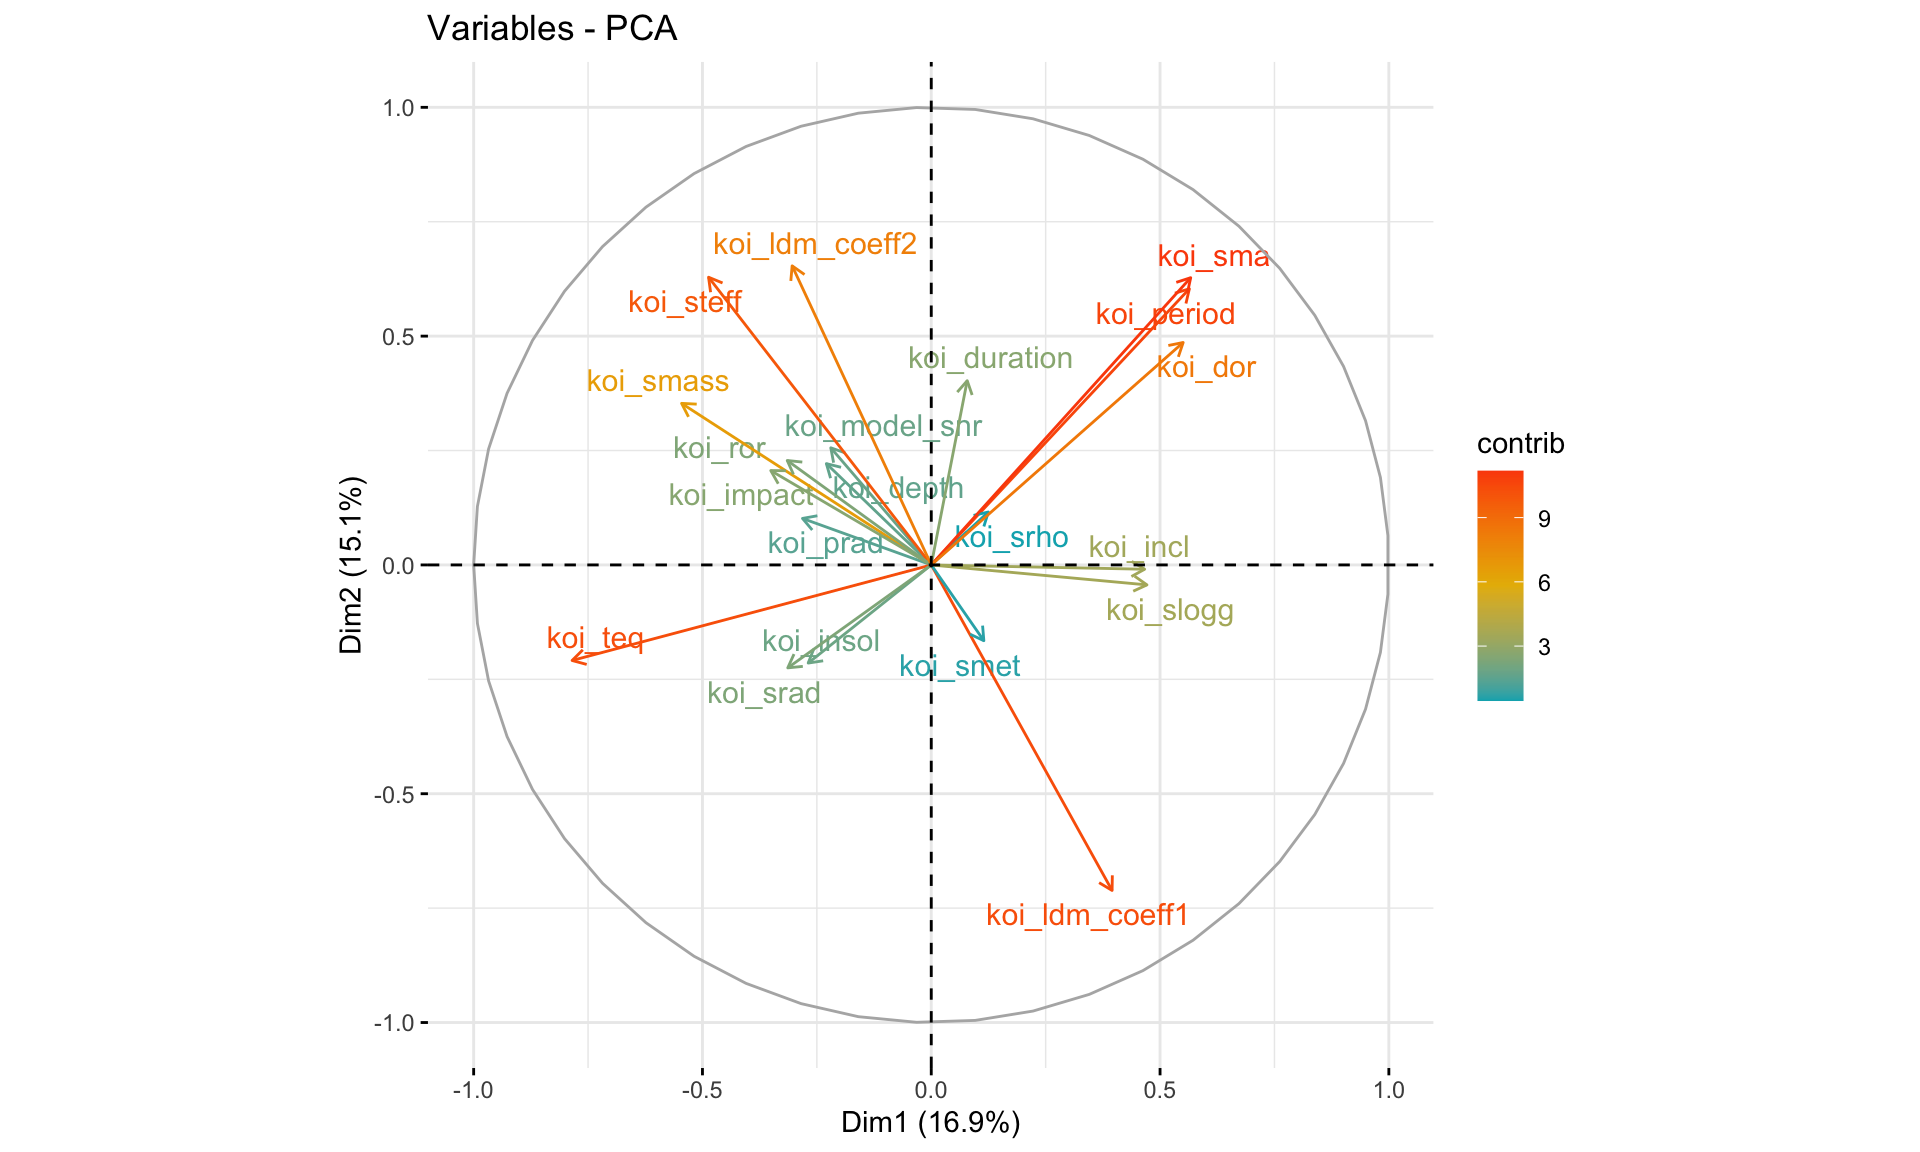
\includegraphics[width=\textwidth]{Immagini/PCA_torta.png}
        \caption{PCA Loadings}
    \end{subfigure}
    \caption{PCA Results}
    \label{fig:pca_plots}
\end{figure}

Figure \ref{fig:pca_plots}-(a) shows that the first two principal components explain only 32\% of the variance, suggesting a complex data structure requiring 11 PCA to capture over 90\% of the variance.

Figure \ref{fig:pca_plots}-(b) shows the loadings of the first two principal components allowing us to understand the relationship between the original variables and the principal components. In general, the loadings analyses report the following:
\begin{itemize}
    \item \textbf{PC1 (17\% variance):} Captures the relationship between orbital characteristics and temperature, showing high positive loadings for orbital parameters (period, semi-major axis, planet-star distance ratio) and negative loadings for equilibrium temperature. Moderate contributions from stellar properties.
    \item \textbf{PC2 (15\% variance):} Primarily represents orbital parameters and stellar temperature relationships, with positive loadings for the orbital period, semi-major axis, and stellar effective temperature, while showing contrasting patterns in limb darkening coefficients.
    \item \textbf{PC3 (14\% variance):} Dominated by stellar characteristics, particularly contrasting stellar radius, and insolation (positive loadings) with surface gravity (negative loading). Orbital parameters show moderate influence.
    \item \textbf{PC4 (12\% variance):} Reflects planetary size and transit geometry, with strong negative loadings for planetary radius, radius ratio, and impact parameter.
    \item \textbf{PC5 (8\% variance):} Represents transit signal characteristics, showing strong negative loadings for transit depth and model signal-to-noise ratio.
    \item \textbf{Later PCs:} Capture more subtle relationships:
    \begin{itemize}
        \item PC6: Transit duration and stellar density
        \item PC7: Insolation and metallicity relationships
        \item PC19/20: Specific period-axis relationships and limb darkening effects
    \end{itemize}
\end{itemize}

These components suggest that the main sources of variation in the dataset are related to transit signal strength, stellar properties, transit geometry, and orbital characteristics.

\section{Models}
Many different models were tested. The following table shows the results of the models tested by comparing their accuracy, AUC (Area Under the ROC Curve), sensitivity, and specificity (see files \texttt{model.rmd} and \texttt{model\_pca.rmd}).
\begin{figure}[H]
    \centering
    \begin{minipage}{0.48\textwidth}
        \centering
        \small
        \setlength{\tabcolsep}{4pt}
        \begin{tabular}{|l|c|c|c|c|}
            \hline
            \textbf{Model} & \textbf{Acc} & \textbf{Sens} & \textbf{Spec} & \textbf{AUC} \\ \hline
            GLM & .819 & .764 & .873 & .888 \\ \hline
            GAM & .827 & .789 & .865 & .893 \\ \hline
            GLM Int. & .750 & .899 & .603 & .751 \\ \hline
            Lasso & .809 & .720 & .896 & .882 \\ \hline
            Ridge & .811 & .730 & .890 & .883 \\ \hline
            RF PCA & .627 & .914 & .330 & .697 \\ \hline
            GLM PCA & .725 & .464 & .979 & .869 \\ \hline
            GAM PCA & .621 & .238 & .993 & .733 \\ \hline
        \end{tabular}
        \caption{Models Performance Comparison}
        \label{tab:model_comparison}
    \end{minipage}
    \hfill
    \begin{minipage}{0.48\textwidth}
        \centering
        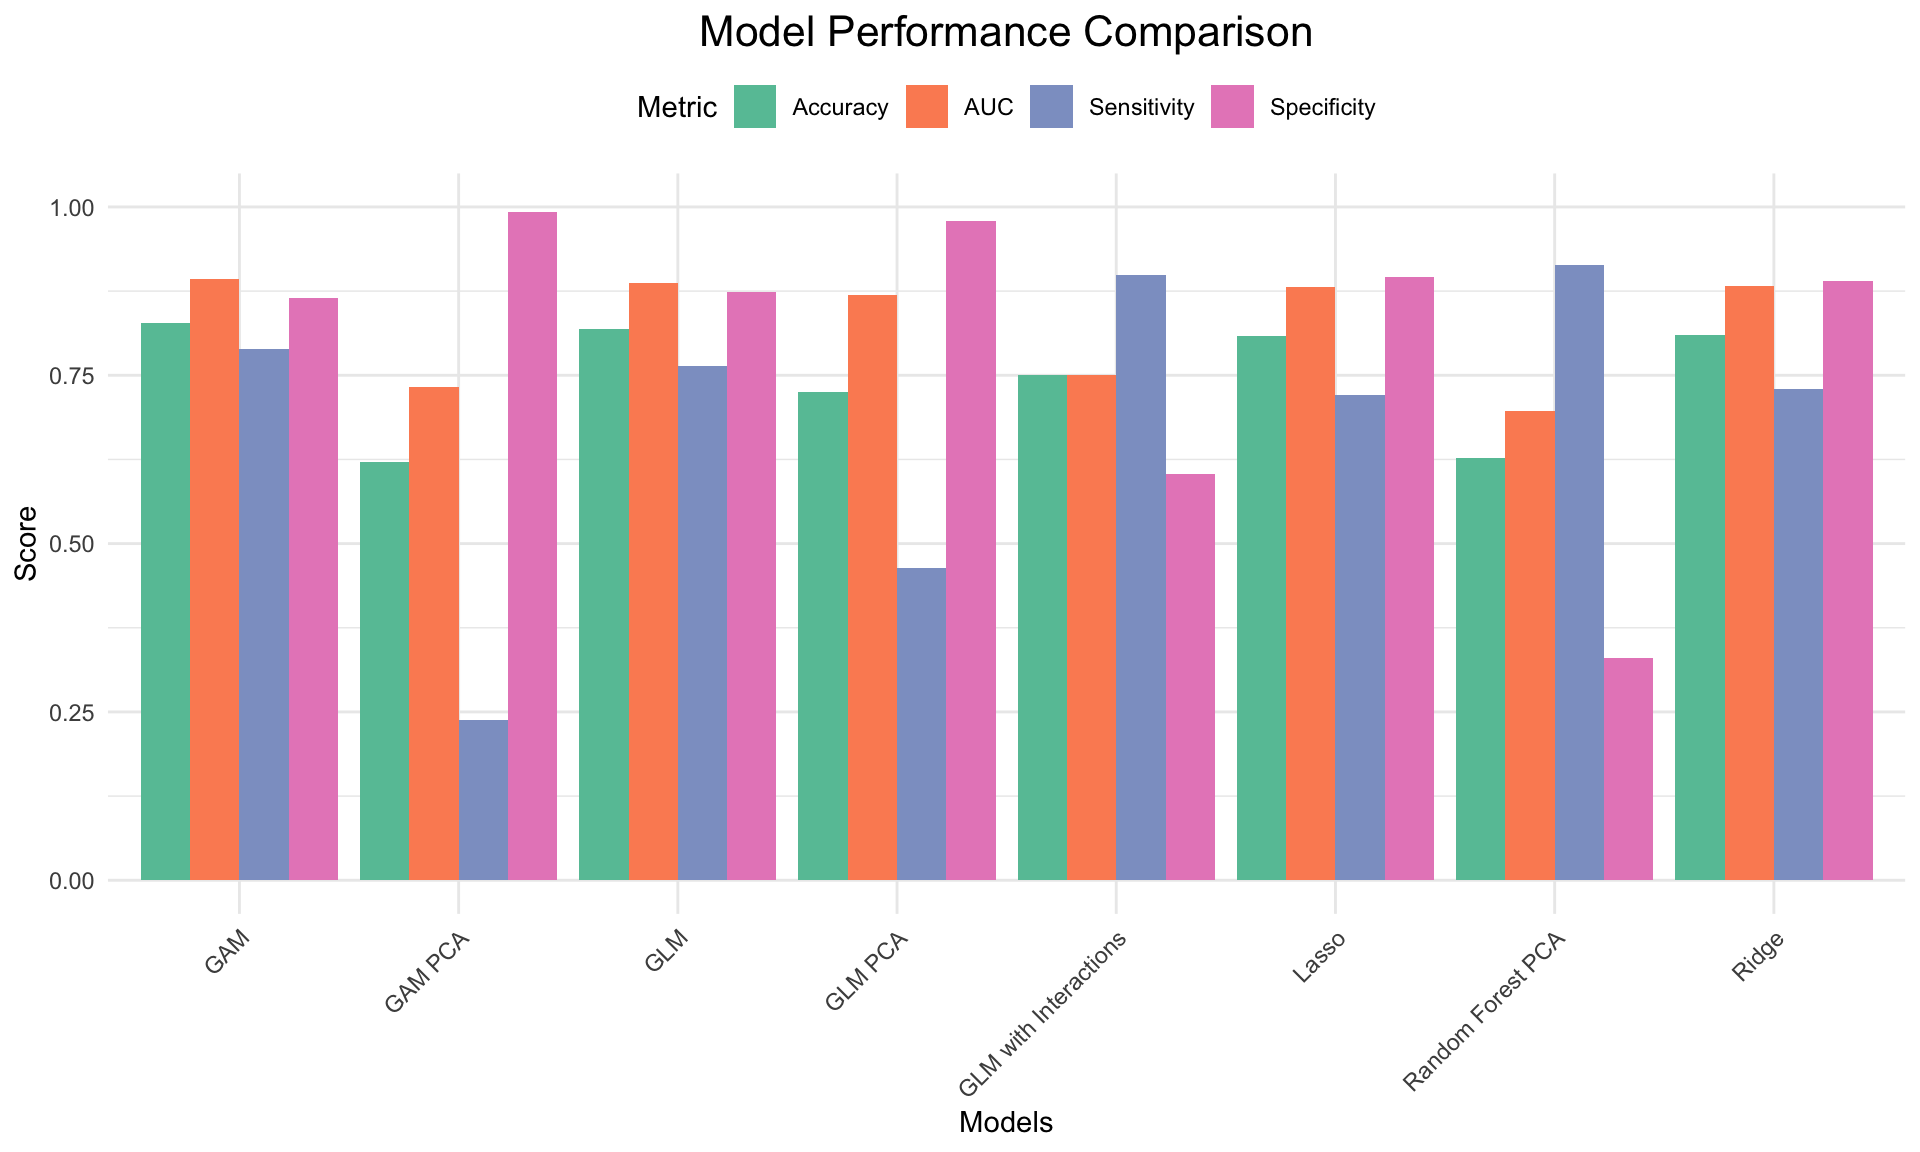
\includegraphics[width=\textwidth]{Immagini/model_comp.png}
        \caption{Visual Comparison of Models Performance}
        \label{fig:models_performance}
    \end{minipage}
\end{figure}

\subsection{Data preprocessing}
The \textbf{null values} in the dataset were \textbf{imputed} after splitting the dataset into train and test sets by applying simple median/mode imputation. This simple but effective approach was chosen because it was the most efficient and because the number of missing values was small for the interested columns.

Also, the numerical columns were \textbf{scaled} before training the models. Also in this case the scaler is trained on the train set and then applied to the test set to avoid data leakage.

\subsection{Outliers and Correlated Features}
For some models, the \textbf{outliers} were \textbf{removed} from the dataset by computing the Cook's Distance for each observation and removing those with a Cook's Distance greater than 0.5. This approach was chosen because it was the most efficient and because the number of outliers was small for the interested columns.

The \textbf{correlated features} were \textbf{removed} from some models by computing the VIF (Variance Inflation Factor) for each feature and removing those with a VIF greater than 10.

\chapter{Conclusions}
\section{Original Features vs. PCA Features}
Models trained directly on the original (scaled) features generally demonstrated superior performance compared to those trained on PCA features in this analysis. The GLM, GAM, Lasso, and Ridge models using original features all achieved AUCs above 0.88, whereas the models using PCA features had lower AUCs (0.70-0.87) and often exhibited extreme trade-offs between Sensitivity and Specificity, potentially influenced by the definition of the positive class during evaluation. This suggests that PCA, as implemented here, might have resulted in some information loss detrimental to predictive performance for this specific task compared to using the original, interpretable features.

\section{Performance Among Original Feature Models}
\begin{itemize}
    \item \textbf{GAM}: The Generalized Additive Model (GAM) emerged as the top performer, achieving the highest AUC (0.8930) and Accuracy (0.8274). It also showed a good balance between Sensitivity (0.7894) and Specificity (0.8648). This suggests that capturing non-linear relationships using smooth functions, as identified in the residual analysis, provided a tangible benefit over the standard linear GLM.
    \item \textbf{Baseline GLM}: the standard GLM performed strongly, with an AUC (0.8875) and Accuracy (0.8193) only slightly below the GAM. It represents a solid baseline.
    \item \textbf{Regularized Models (Lasso \& Ridge)}: Lasso (AUC 0.8816) and Ridge (AUC 0.8828) performed very similarly to each other and slightly below the baseline GLM and GAM in terms of AUC and Accuracy. However, they achieved the highest Specificity values (0.8958 and 0.8896, respectively). This indicates that regularization helped in correctly identifying the negative class (likely candidate if false positive was positive), potentially by handling collinearity or simplifying the model, but at the cost of slightly lower Sensitivity compared to GLM/GAM.
    \item \textbf{GLM with Interactions}: The specific interaction terms added in this test significantly degraded performance (AUC 0.7510, Accuracy 0.7498), particularly hurting Specificity. This suggests the chosen interactions were not beneficial and may have led to overfitting or were not representative of the true underlying relationships.
\end{itemize}

\section{Overall Conclusions}
Based on these results, the GAM using the original scaled features stands out as the most promising model, offering the best balance of overall predictive power (highest AUC and Accuracy) while effectively modeling the non-linearities present in the data.

The standard GLM, Ridge, and Lasso models also provide competitive performance and could be considered strong alternatives, especially if model simplicity (Lasso potentially performs feature selection) or high Specificity (Ridge/Lasso) is prioritized. Further tuning of the prediction probability threshold for any of these top models (GAM, GLM, Ridge, Lasso) could optimize the balance between Sensitivity and Specificity based on specific application requirements (e.g., minimizing false negatives vs. minimizing false positives). The PCA-based approaches and the tested interaction GLM appear less effective based on this comparison.

